\documentclass{article}
\usepackage{tikz}
\usetikzlibrary{shapes.geometric, arrows}

\tikzstyle{startstop} = [rectangle, rounded corners, minimum width=3cm, minimum height=1cm,text centered, draw=black, fill=red!30]
\tikzstyle{process} = [rectangle, minimum width=3cm, minimum height=1cm, text centered, draw=black, fill=orange!30]
\tikzstyle{decision} = [diamond, minimum width=3cm, minimum height=1cm, text centered, draw=black, fill=green!30]
\tikzstyle{arrow} = [thick,->,>=stealth]

\begin{document}

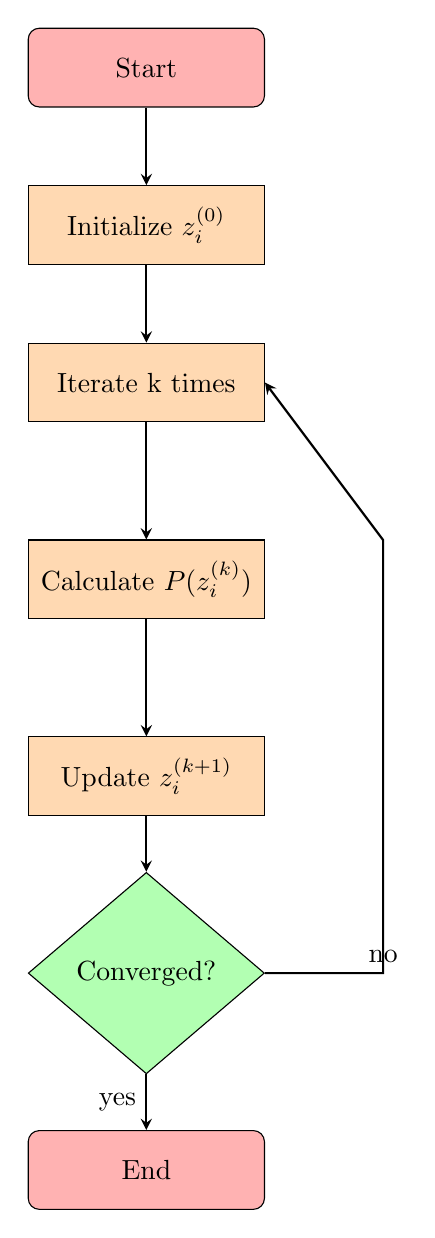
\begin{tikzpicture}[node distance=2cm]

\node (start) [startstop] {Start};
\node (init) [process, below of=start] {Initialize \(z_i^{(0)}\)};
\node (iterate) [process, below of=init] {Iterate k times};
\node (calc) [process, below of=iterate, yshift=-0.5cm] {Calculate \(P(z_i^{(k)})\)};
\node (update) [process, below of=calc, yshift=-0.5cm] {Update \(z_i^{(k+1)}\)};
\node (check) [decision, below of=update, yshift=-0.5cm] {Converged?};
\node (end) [startstop, below of=check, yshift=-0.5cm] {End};

\draw [arrow] (start) -- (init);
\draw [arrow] (init) -- (iterate);
\draw [arrow] (iterate) -- (calc);
\draw [arrow] (calc) -- (update);
\draw [arrow] (update) -- (check);
\draw [arrow] (check) -- node[anchor=east] {yes} (end);
\draw [arrow] (check.east) -- ++(1.5,0) node[anchor=south] {no} -- ++(0,5.5) -- (iterate.east);

\end{tikzpicture}

\end{document}